\chapter{Keeping Information Secret}
\label{chapter:keepingInformationSecret}

The previous chapter \ref{chapter:representing_information_with_symbols} was about representing information with symbols. This section is about keeping information secret.
Ciphers haven been used for thousands of years \cite{HistoryOfCryptography}. They are used to keep information secret from people, that are not supposed to have knowledge of it. Not encrypted information is called clear text. Once one encrypted a clear text, it is called a cipher text and only people who know how to decrypt the cipher text can read originally encrypted information.
The exercises in this section are introducing pupils to the concepts of ciphers.

\section{Cipher Texts from Reversed Letters}
\label{section:patterns}

\subsection{Exercises}
The cipher used in these exercises is a simple mix up of letters and both directions are trained: encryption and decryption. In the decryption exercise, the pattern, on which the clear text was encrypted with, is shown. The pupils need to understand the pattern and move the letters in the cipher text accordingly to retrieve the clear text. The encryption exercise is set up analogously. Multiple difficulty levels are possible by changing the amount of moved letters.

\begin{example}
    The cipher text is \code{ULFSS} and the pattern is shown in figure \ref{fig:pattern}. By moving the letter in the cipher text according to the pattern, the clear text can be retrieved: \code{FLUSS}.
\end{example}

\begin{figure} 
    \centering
    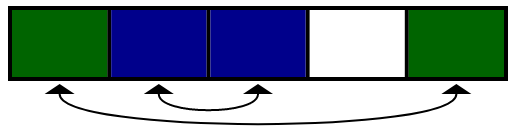
\includegraphics[width=0.4 \columnwidth]{figures/pattern.png}
    \caption{Pattern} 
    \label{fig:pattern} 
\end{figure}

\subsection{Implementation}

Both exercises have a similar Implementation. Both need drawn pattern that indicates the cipher. Fundamentally, the only difference is that for the decryption exercise the given text consists of reverser letters and the solution is compared to the original word, while the encryption exercise gives first the original word as a text and the solution is compared to match the pattern. 
The pattern is created by generating an array of tuples. Each tuple indicates two swapped letters. These two letters are selected randomly and have to be distinct. The exact algorithm used is given in Listing \ref{lst:createPattern}.
Both encryption and decryption exercises have two difficulty levels. They differ by the amount of tuples

\begin{itemize}
    \item \textbf{easy} - one tuple i.e two swapped letters 
    \item \textbf{medium} - two tuples, i.e in total four swapped letters if the the word has at least four letters, otherwise only two swapped letters 
\end{itemize}

%TC:ignore
\begin{lstlisting}[language=TypeScript,caption={Algorithm to generate an array of distinc tuples of given size},label={lst:createPattern}]
createPattern(text: string[], swapAmount: number): Array<[number, number]> {
  const pattern = new Array<[number, number]>();
  const letters = [...Array(text.length).keys()];
  for (let j = 1; j <= swapAmount && 2 * j <= text.length; j++) {
    const leftIndex = Math.floor(Math.random() * letters.length);
    const left = letters[leftIndex];
    letters.splice(leftIndex, 1);
    const rightIndex = Math.floor(Math.random() * letters.length);
    const right = letters[rightIndex];
    letters.splice(rightIndex, 1);
    pattern.push([Math.min(left, right), Math.max(left, right)]);
  }
  return pattern;
}
\end{lstlisting}
%TC:endignore

The array of tuples needs to be graphically represented. 
\TODO{explain canvas}
Drawing the pattern on a canvas requires four steps: 

\begin{itemize}
  \item \textbf{drawing the grid} - each cell represents a letter of the word
  \item \textbf{colorizing the pairs} - the pairs representing the two letters that need to be swapped are colorize in the same color
  \item \textbf{drawing the arrow heads} - underneath each cell that is part of a pair a arrow head is drawn
  \item \textbf{drawing the arrow lines} - connecting the pairs with lines without the lines crossing or overlapping each other
\end{itemize}

The implementation for these steps is given in Listing \ref{lst:createPattern}.
\TODO{maybe show how the arrow levels are calculated}

%TC:ignore
\begin{lstlisting}[language=TypeScript,caption={Implementation to draw the pattern on a canvas element},label={lst:drawPattern}]
drawPattern(cells: number, pairs: [number, number][]) {
  const rectX = this.lineWidth / 2;
  const rectY = this.lineWidth / 2;
  const rectWidth = this.width - this.lineWidth;
  const cellHeight = this.height / 2 - this.lineWidth;
  const cellWidth = rectWidth / cells;

  this.drawGrid(rectX, rectY, rectWidth, cellHeight, cells, cellWidth);

  // sort to have it easier to draw the lines connecting the boxes on the correct height
  pairs.sort(([a, b], [c, d]) => Math.abs(a - b) - Math.abs(c - d));
  const arrowLevelY = this.calculateArrowLevelY(pairs);
  for (let i = 0; i < pairs.length; i++) {
    for (let j = 0; j < 2; j++) {
      const pairIndex = pairs[i][j];

      this.ctx.fillStyle = this.colors[i % this.colors.length];
      this.fillBox(rectX, rectY, cellHeight, cellWidth, pairIndex);

      const centerX = rectX + cellWidth * pairIndex + cellWidth / 2;
      this.ctx.fillStyle = "black";
      this.drawArrowHead(
        centerX,
        rectY + cellHeight + 5,
        Math.min(30, cellWidth),
        10
      );
    }

    this.drawArrowLine(
      cellHeight,
      cellWidth,
      rectY,
      rectX,
      arrowLevelY.get(JSON.stringify(pairs[i])),
      cells,
      pairs[i]
    );
  }
}
\end{lstlisting}
%TC:endignore

\section{Cipher Texts from New Characters}
\label{section:symbols}

\subsection{Exercises}
Sometimes, only moving symbols in not enough to keep information secret. A better why is to substitute symbols with new symbols. These symbols may be letters, numbers or completly new symbols, that are solely invented for the purpose of encrypting information.
In the following exercises the last approach is followed. Again both direction, encryption and decryption, are trained. But this time, instead of having a pattern, there is a symbol table showing how the letters are encrypted. 

\begin{example}
    The cipher text is shown in figure \ref{fig:cipher_number} and the symbol table in figure \ref{fig:symbol_table}. By using the symbol table one can decrypt the cipher text to \code{52}.
\end{example}

\begin{figure} 
    \centering
    
\includegraphics[width=0.2 \columnwidth]{figures/cipher_number.png}
    \caption{Cipher text of an encrypted number} 
    \label{fig:cipher_number} 
\end{figure}

\begin{figure} 
    \centering
    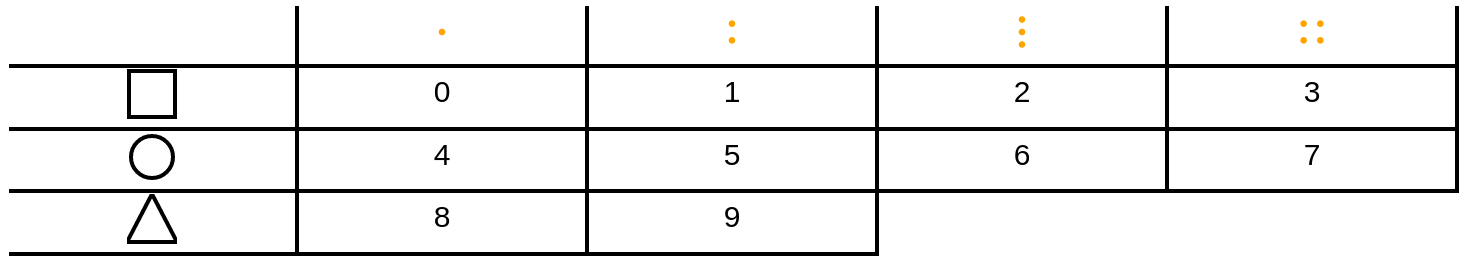
\includegraphics[width=1.0 \columnwidth]{figures/symbol_table.png}
    \caption{Symbol table to encrypt numbers} 
    \label{fig:symbol_table} 
\end{figure}

\subsection{Implementation}

% draw encrypted 
% symbol table

